Referring to \cref{fig:ev-poly-n5}, for a point  $P\in\EE$ 
define $\PP_u = P + u (C-P)$, where $u$ is a scalar and
$C$ is the center of the curvature
(i.e. the center of the circle osculating $\EE$ in $P$).
For fixed $u$ the map $P\mapsto \PP_u$ sends $\EE$
to the ``evolute curve'' $\EE_u$,
e.g. if $\EE_0 = \EE$ and $\EE_1$ is the evolute (i.e. the curve swapped by the centers of curvature).
Similarly vertices of the ``evolute polygons'' are defined as the images of
the vertices of affine-regular polygons.

Over $\FF$, the area $\AA_u$ of $\PP_u$ is constant, for all $N{\neq}1,2,4$. It is given by:
\begin{equation}
\small
\label{:as}
\frac{\AA_u}{N} = \frac{1}{32 a b}
\left[{{\left((a^2 + 3\,b^2)\cdot u- 4\,a^2 \right)
\left( (3\,a^2+b^2)\cdot u - 4\,b^2 \right) } \sin(α) }
+  u^2 c^4 \cdot \sin(3α)\right]
\end{equation}
 
\begin{proof}
The coordinates of $C$ (and hence of $\PP_u$)
are cubic trigonometric polynomials, odd with respect to the total grading.
{\color{red} In initial sections I have not described the total grading,
described only another one, that we do not really use.}
Therefore the area $A_u(P) = \frac{\PP_u\wedge \mathcal{ρ(P)}_u}2$
is an even Laurent polynomial of degree at most $6$.
In fact the highest degree terms of $\PP_u$ and $\mathcal{ρ(P)}_u$
are proportional, so $A_u(P)$ is an even Laurent polynomial of degree $4$.
Apply \cref{:Laurent} and compute $\AA_u := T_0 A_u$.
\end{proof}

\noindent The variation of $\AA_u$ for quadrangles is illustrated in \cref{fig:ev-poly-n4}.

\begin{corollary}
For every $N$ there are two values of $u$ such that $\AA_u = 0$.
\end{corollary}
\begin{proof}
\cref{:as} is quadratic in $u$: by definition $\PP_u$ and $\mathcal{ρ(P)}_u$
are linear in $u$ and wedge product is bilinear.
\end{proof}

\noindent \cref{fig:ev-poly-zero-area} illustrates null $\AA_u$ for $N\leq7$.
Referring to \cref{fig:zero-n3}:

\begin{observation}
%For the $N=3$ case, the area of $\AA_s$ is given by:
%\[{\frac { \sqrt {3} \left( 9\,{a}^{2}+3\,{b}^{2} \right) \left( {a}^{2}+3\,{b}^{2} \right) {u}^{2}}{64\,a\, b}}-{\frac {\sqrt {3} \left( 9\,{a}^{4}+6\,{b}^{2}{a}^{2}+9\,{b}^{4} \right) u}{16\,a \,b}}+{\frac {3\,\sqrt {3}\; a b}{4}}\]
For triangles, $\AA_u=0$ for $u=4b^2/(3a^2 + b^2)$ or $u=4a^2/(a^2 + 3b^2)$;
in each case, the vertices of $\PP_u$ are collinear and parallel to the axes of either ellipse.
\end{observation}

Indeed, as shown on this \href{https://youtu.be/OFA_j25R8ks}{Video}, these two segments meet at the {\em 3rd Brocard point} of the triangle \cite[X(76)]{etc}.

\begin{observation}
Only for triangles and quadrangles, the family of $\PP_u$ has constant sum of cotangents, for all $u$.
Note that for triangles this sum is not defined if $\AA_u=0$ (a segment has $3$ null angles);
for quadrangles said sum is equal to zero (family of parallelograms).
\end{observation}

Referring to \cref{fig:zero-area-inf}, when $Ν{\rightarrow}\infty$ (more generally, $α\rightarrow 0$ or $ζ\rightarrow 1$),
\begin{equation}
\label{eqn:ninf}
\lim_{α\to 0}
\frac{\AA_u}{πab} = 1 - \frac {\, \left( 3\,{a}^{4}+2\,{a}^{2}{b}^{2}+3\,{b}^{4} \right)}{8\,a^2\, b^2} \cdot u (2-u).
\end{equation}
%\textcolor{red}{ronaldo $\AA_s=...$ at $u=...$. These curves are known as ... or have degree ...}.

\begin{figure}
    \centering
    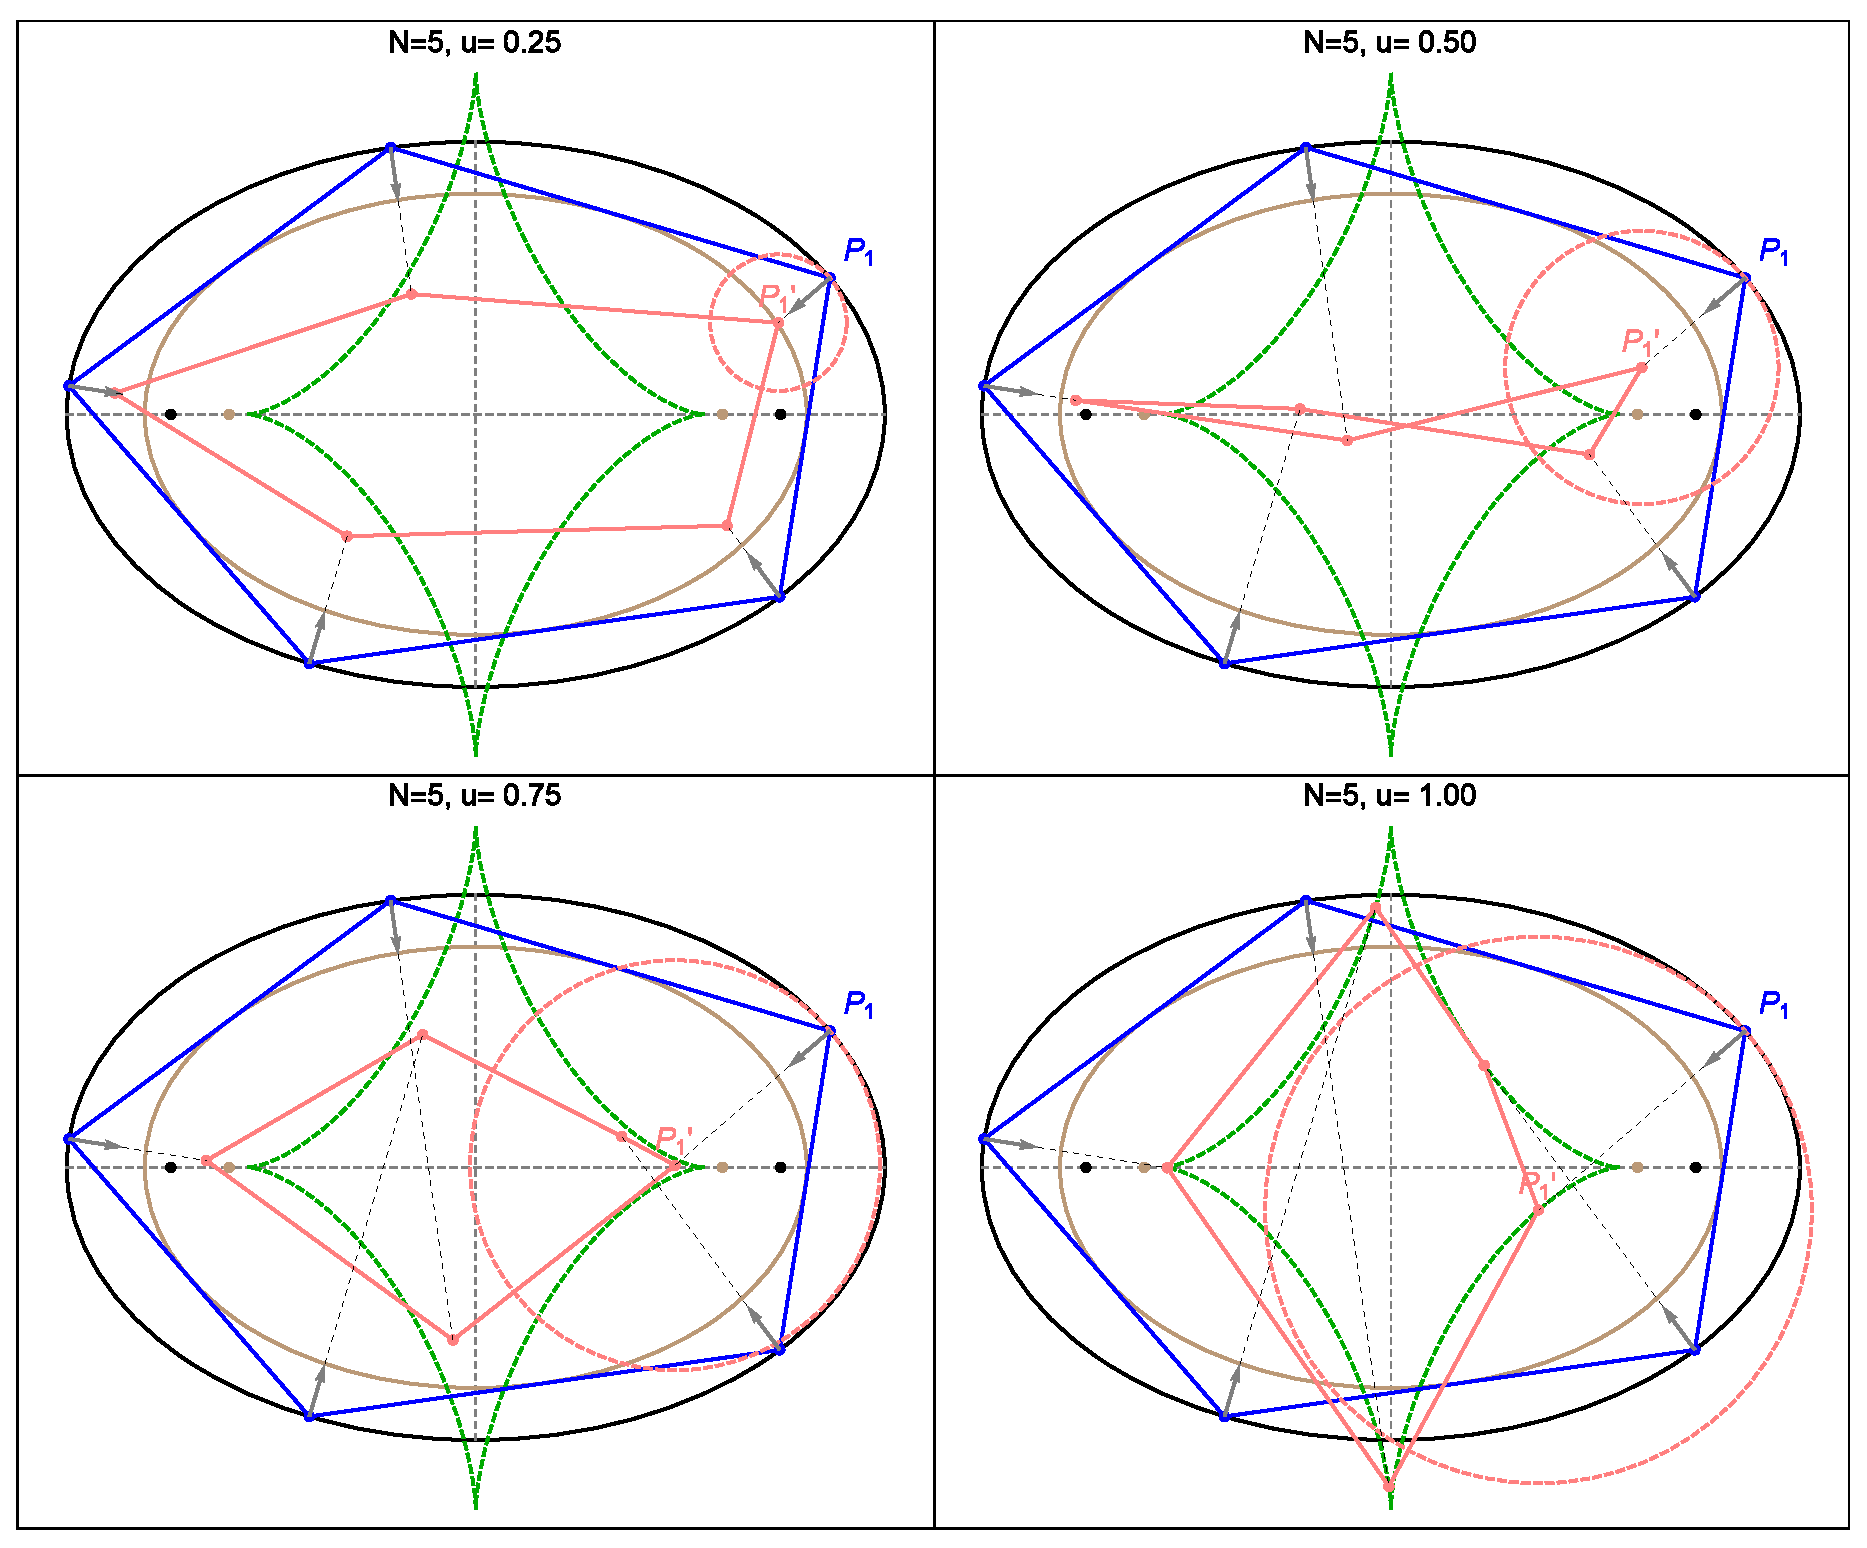
\includegraphics[width=\textwidth]{pics/0070_evolute_poly_n5.eps}
    \caption{Constant signed-area evolute pentagons (pink) for various values of $u$. The outer ellipse has $a/b=3/2$. The dashed circle centered on $P_1'$ and passing through $P_1$ has radius $u R_1$ where $R_1$ is the inverse curvature at $P_1$. Notice that when $u=1$ (bottom right), the $P_i'$ lie on the evolute (dashed green). \href{https://youtu.be/JCj0q7_hlA8}{Video}}
    \label{fig:ev-poly-n5}
\end{figure}

\begin{figure}
    \centering
    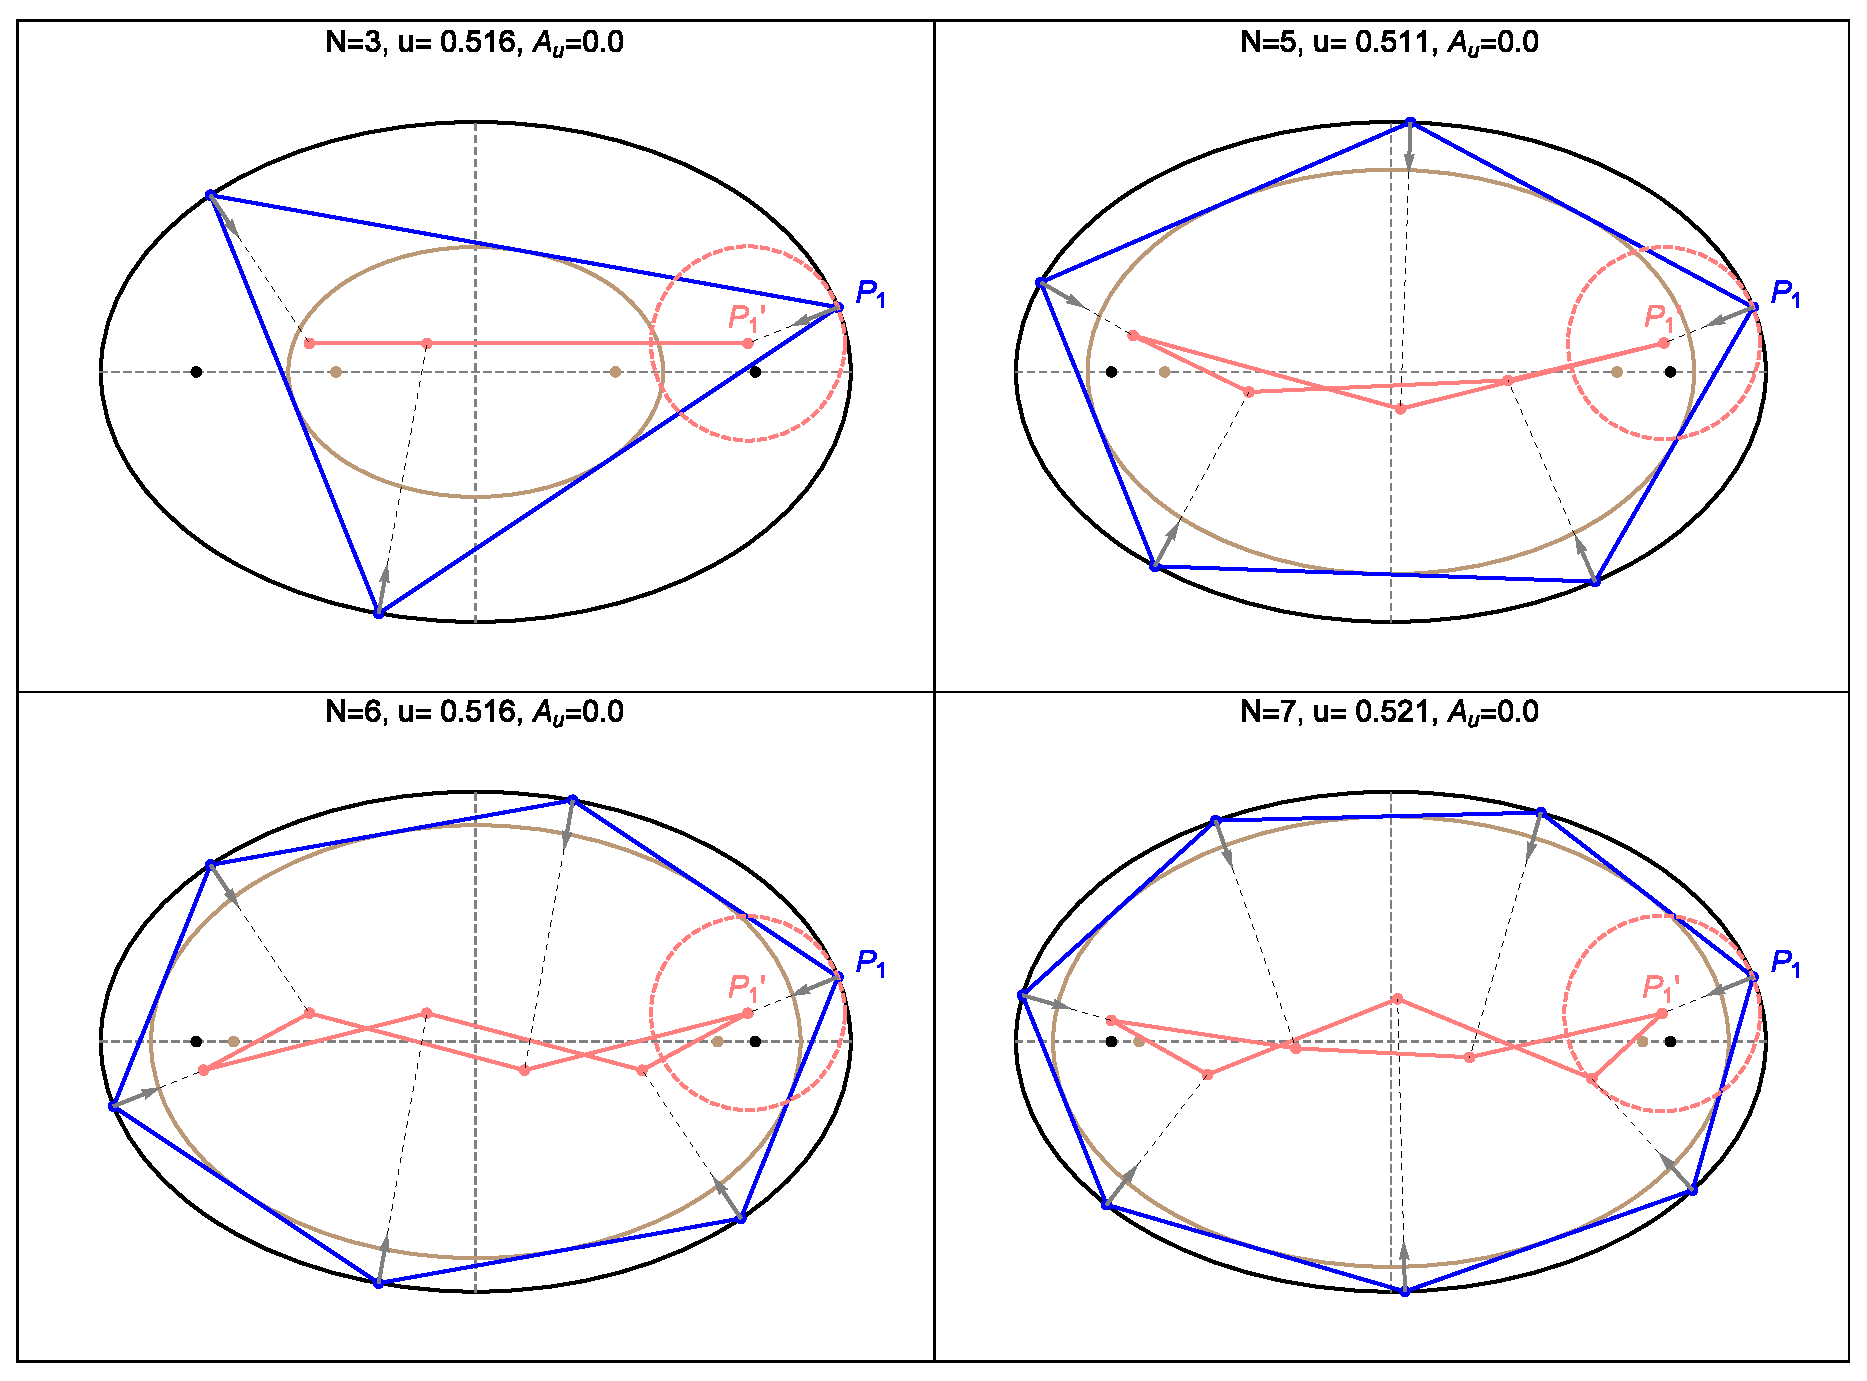
\includegraphics[width=\textwidth]{pics/0080_evolute_poly_zero_area.eps}
    \caption{Zero-area evolute triangles, pentagons, hexagons and septagons (pin) inscribed in an ellipse with $a/b = 3/2$.
             Quadrangles are omitted as for all $u$, its area is variable. \href{https://youtu.be/3nvXYFoI5Wg}{Video}.}
    \label{fig:ev-poly-zero-area}
\end{figure}

\begin{figure}
    \centering
    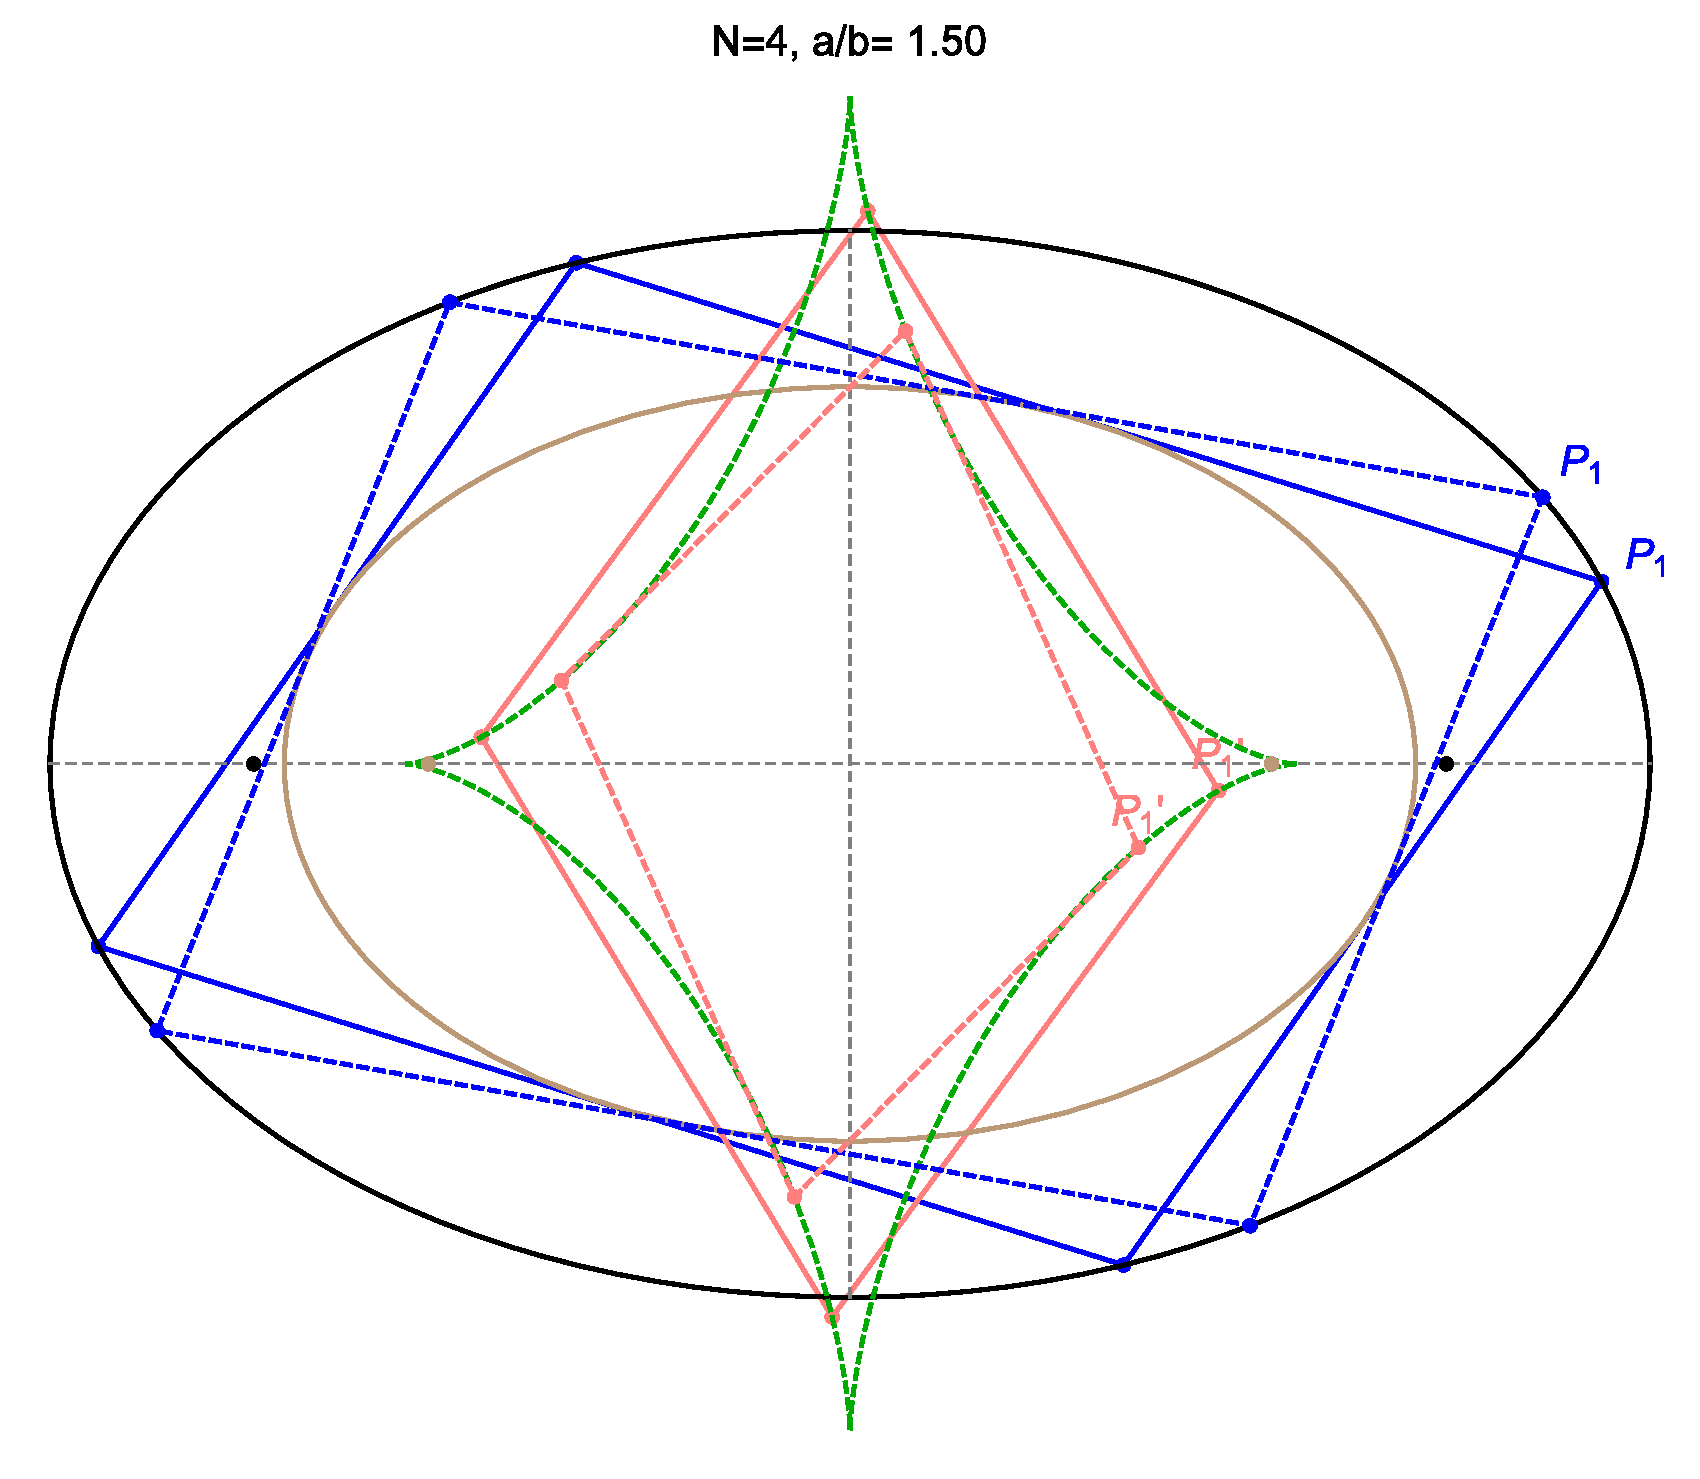
\includegraphics[width=.7\textwidth]{pics/0050_n4_ev_poly.eps}
    \caption{Two quadrangles (blue and dashed blue) and their respective evolute polygons $\PP_u$ (pink, dashed pink), for $u=1$.
             Exclusively for quadrangles, $\AA_u$ is variable, for any $u$ chosen.
             Note that the $T_N u^2$ is variable for both quadrangles and hexagons.
             {\color{red} If variables for hexagons shall be variable for triangles as well, cf \cref{:functoriality}.}
             }
    \label{fig:ev-poly-n4}
\end{figure}


\begin{figure}
    \centering
    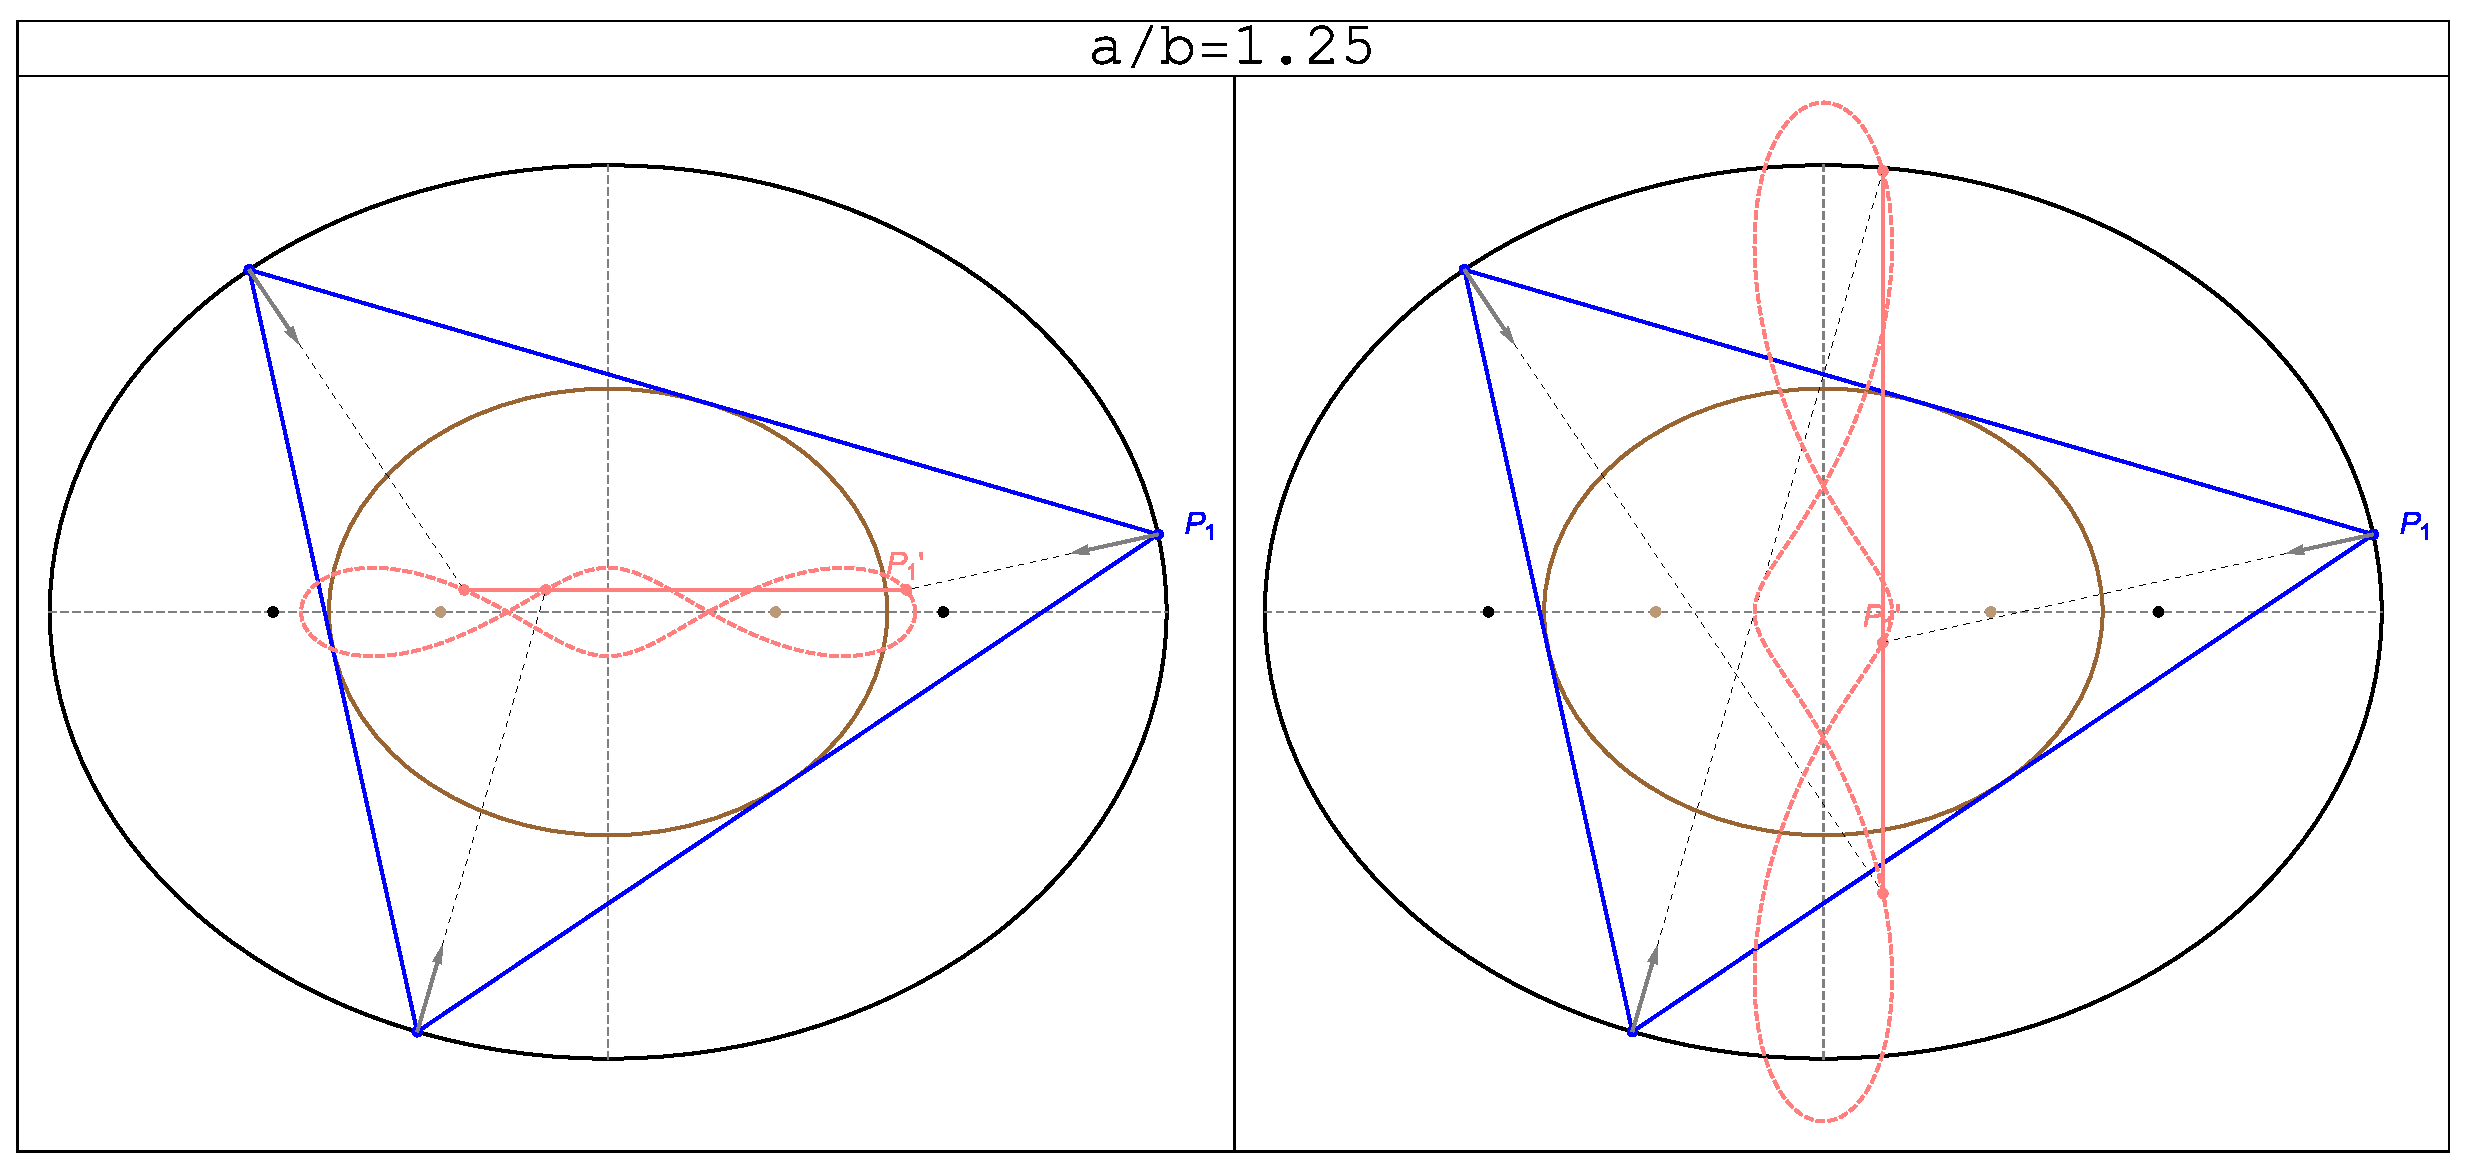
\includegraphics[width=\textwidth]{pics/0090_zero_area_n3_both.eps}
    \caption{The two zero-area evolute triangles are segments parallel to either axes of the ellipses.
             Also shown is the self-intersected locus of their vertices. \href{https://youtu.be/f80QaYs5_J4}{Video 1}.
             It turns out the two segments meet at the triangle center named $X_{76}$ \cite{etc} \href{https://youtu.be/OFA_j25R8ks}{Video2}.}
    \label{fig:zero-n3}
\end{figure}

\begin{figure}
    \centering
    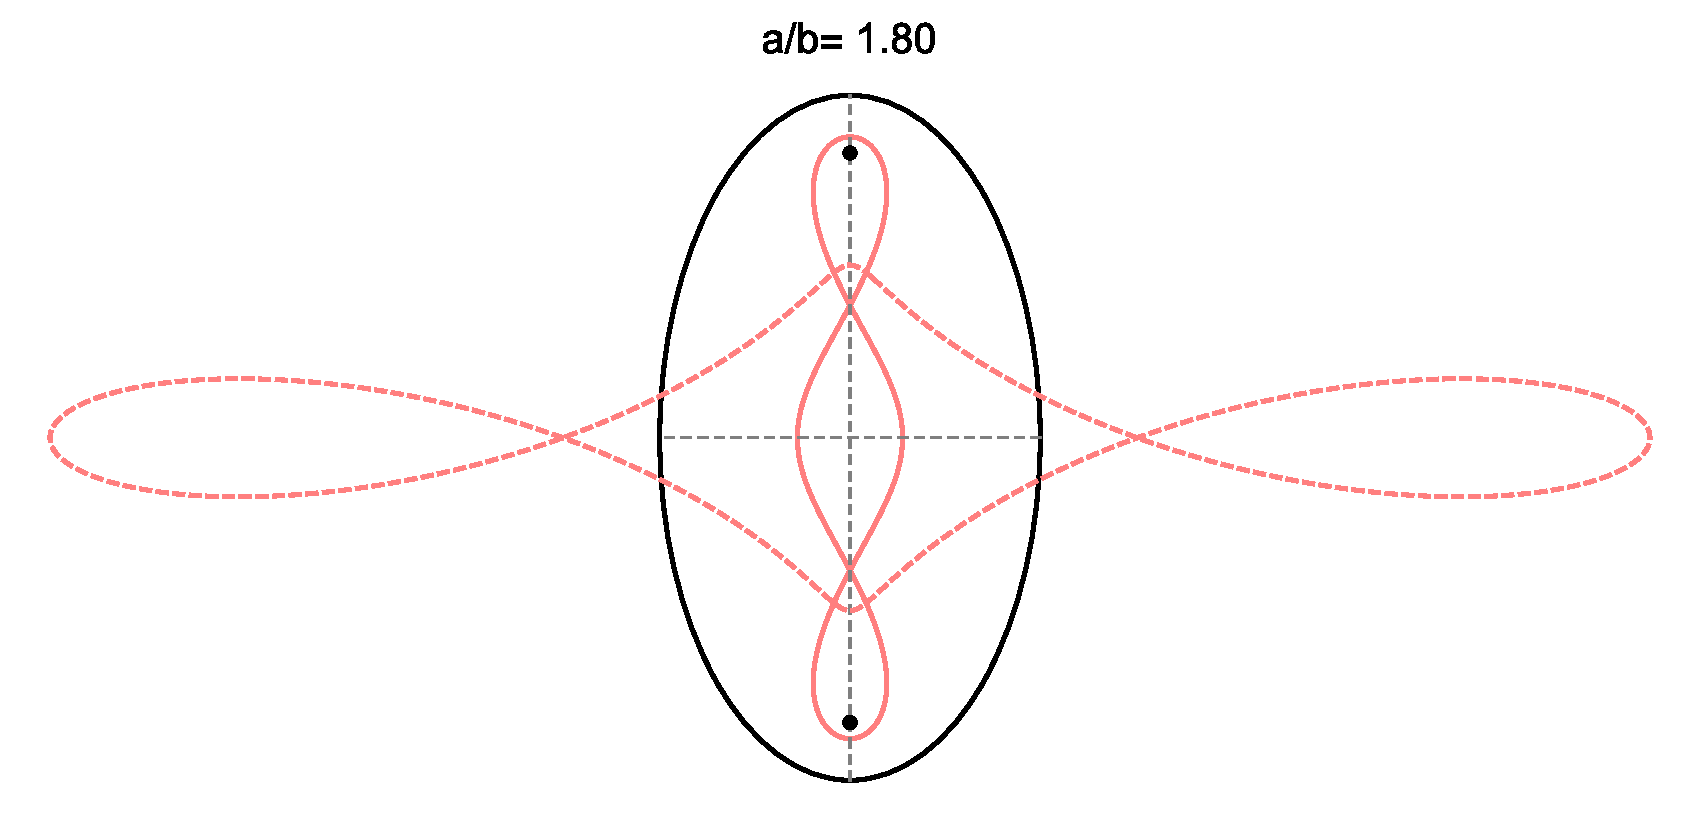
\includegraphics[width=.7\textwidth]{pics/0100_zero_area_ninf_both.eps}
    \caption{The two zero-area evolute polygons (pink and dashed pink) when $N$ is infinite, see \cref{eqn:ninf}.}
    \label{fig:zero-area-inf}
\end{figure}

Note when $u=0$, $\PP_u$ is the original polygon, and the sum of its squared sidelengths is a constant given in \cref{:sqr_si}.

Let $\ell_i$ denote the $i$-th sidelength of $\PP_u$.

If $s{\neq}0$ and $N{\notin}\{1,2,3,4,6\}$, the trace $T_N \ell^2$ is a constant equal to:
{\small  
\begin{equation}
\label{:ell2}
 2 \sin^2\left(\frac{α}{2}\right) \left[ \frac{c^4 u^2}{2}\left ( \cos α \cos^2\left(\frac{α}{2}\right) \right) +\frac{u^2}{8}( 5a^4  - 2a^2b^2  +  5b^4 )  - a^2b^2(2 u - 1)\right] \frac{ a^2+b^2}{a^2 b^2}
\end{equation}

\begin{equation}\aligned
 & - \,{\frac {{u}^{2} \left( {a}^{2}-{b}^{2} \right) ^{2} \left( {a}^
{2}+{b}^{2} \right) }{16{a}^{2}{b}^{2}}}\cos 3\alpha\\
&-\left( \,{\frac { \left( 9\,{a}^{4}-2\,{a}^{2}{b}^{2}+9\,{b}^{4}
 \right)  \left( {a}^{2}+{b}^{2} \right) {u}^{2}}{16{a}^{2}{b}^{2}}}+
 \left( {a}^{2}+{b}^{2} \right)  \left( 1-2\,u \right) 
\right)\cos\alpha\\
&+\frac { \left( 5\,{a}^{4}-2\,{a}^{2}{b}^{2}+5\,{b}^{4} \right) 
 \left( {a}^{2}+{b}^{2} \right) {u}^{2}}{8{a}^{2}{b}^{2}}+ \left( {a}^
{2}+{b}^{2} \right)  \left( 1-2\,u \right) 
\endaligned
\end{equation}

%\textcolor{green}{ron: done}
%{\color{red} Simplify the formula. All entities like $\sin^2(α/2)$, $\cos^2(α/2)$ can be given in terms of $\sin(α)$, $\cos(α)$.
%Compare with the script that computes everything in terms of powers of $ζ$(named $w$),
%i.e. in terms of $\cos(nα)$ and $\sin(nα)$ with $n$ integer. }
}
\begin{proof}
Similar to the case of \cref{:as}, but without cancellation of the leading terms,
so $\ell^2$ is an even trigonometric polynomial of degree six with non-vanishing
fourth coefficient, the cases $N=1,2,3$ are impossible thanks to \cref{:functoriality}. %Note that for $N=3$ the quantity isn't constant because $N\neq 6$ implies $N\neq3$.
\end{proof}
